%!TEX program = xelatex
%!TEX root = ./thesis.tex
\appendix

\chapter{Miscellaneous IAQI Standards}\label{chapter:IAQI_standards}

This appendix section lists a complete data preprocessing results

It uses the same way to map concentration data into IAQI, and finally calculates AQI, the only different is the thresholds. Both USA and China use the maximum IAQI to represent final AQI.

According to Technical Regulation on Ambient Air Quality Index (on trial) \cite{regulation2012} release by former Ministry of Environmental Protection of the People's Republic of China, IAQI (individual air quality index) and AQI (air quality index) should be calculated by the following equations:

\begin{equation}
    IAQI_p = \frac{IAQI_{Hi}-IAQI_{Lo}}{BP_{Hi}-BP_{Lo}}(C_p-BP_{Lo})+IAQI_{Lo}
\end{equation}

or equivalently:

\begin{equation}
    \label{formula:IAQI_appendix1}
    IAQI_p = \frac{C_p-BP_{Lo}}{BP_{Hi}-BP_{Lo}}(IAQI_{Hi}-IAQI_{Lo})+IAQI_{Lo}
\end{equation}

In formula \ref{formula:IAQI_appendix1}, $C_p$ is the concentration value for certain category like $PM_{2.5}$; $BP_{Hi}$ and $BP_{Lo}$ are high threshold/low threshold near $C_p$, respectively; $IAQI_{Hi}$ and $IAQI_{Lo}$ are high threshold/low threshold $C_p$, respectively.

Then calculate AQI by making use of the maximum of these individual IAQI values \ref{appendix:formula:AQI}:

\begin{equation}
    \label{appendix:formula:AQI}
    AQI = \max\{IAQI_1,IAQI_2,IAQI_3,...,IAQI_n\}
\end{equation}

For each pollutant category, concentration value will firstly all be mapped into the IAQI value according to its corresponding thresholds in the thresholds table \ref{table:IAQI-thresholds}.

The regulation \cite{regulation2012} determines concentration value thresholds for pollutant categories such as $SO_2$, $NO_2$, $CO$, $PM_{2.5}$, $PM_{10}$ and $O_3$. For one-hour average value and 24-hour average value, thresholds are determined differently, for $SO_2$, $NO_2$, $CO$. Note that the thresholds for $PM_{2.5}$ and $PM_{10}$ concentration value are defined by their 24-hour average, this means the method of calculating IAQI for a single day. However, it doesn't matter when we uses these thresholds for realtime (1 Hz) $PM_{2.5}$ and $PM_{10}$ concentration data. Table \ref{table:IAQI-thresholds} shows the $PM_{2.5}$ and $PM_{10}$ data-IAQI mapping relationship. Followed by data we could collect in our AIoT system, we only consider $PM_{2.5}$ and $PM_{10}$ data.

\begin{table}[!htbp]
    \centering
    \caption{Concentration thresholds of IAQI with regard to pollutant categories, China}
    \label{table:IAQI-thresholds}
    \begin{tabular}{|l|l|l|}
    \hline
    IAQI & $PM_{2.5}$ ($\mu g/m^3$) & $PM_{10}$ ($\mu g/m^3$) \\ \hline
    0    & 0   & 0   \\ \hline
    50   & 35  & 0   \\ \hline
    100  & 75  & 150 \\ \hline
    150  & 115 & 250 \\ \hline
    200  & 150 & 350 \\ \hline
    300  & 250 & 420 \\ \hline
    400  & 350 & 500 \\ \hline
    500  & 500 & 600 \\ \hline
    \end{tabular}
\end{table}

Use the formula and table above, we can plot in Figure \ref{fig:iaqi} the value-IAQI mapping curve for both $PM_{2.5}$ and $PM_{10}$. This is a visualization for the air pollutant concentration and its IAQI. For each category, data vary from 0 to 800, linearly.

\begin{figure}[!htbp]
    \centering
    \includegraphics[width=0.7\linewidth]{fig/iqai.pdf}
    \caption{IAQI curve of $PM_{2.5}$ (orange line) and $PM_{10}$ (green line) data.}
    \label{fig:iaqi}
\end{figure}

For data we collected, following the the IAQI thresholds table, each data of a pollutant category are mapped into IAQI values and have six levels, level 1 to 6. In USA's Technical Assistance Document \cite{daq2018} level 1 to 6 of the air quality index is represented by color \colorbox{green}{green}, \colorbox{yellow}{yellow}, \colorbox{orange}{orange}, \colorbox{red}{red}, \colorbox{purple}{purple} and \colorbox{maroon}{maroon}, respectively. We mapped our $PM_{2.5}$ and $PM_{10}$ data into IAQI respectively, as Figure \ref{fig/pm25_all_iaqi} and Figure \ref{fig/pm10_all_iaqi} shows.

\begin{figure}[!htbp]
    \begin{center}
    \includegraphics[width=\linewidth]{fig/iaqi/pm25_all_iaqi.png}
    \end{center}
    \caption{All $PM_{2.5}$ IAQI data.}
    \label{fig/pm25_all_iaqi}
\end{figure}

\begin{figure}[!htbp]
    \begin{center}
    \includegraphics[width=\linewidth]{fig/iaqi/pm10_all_iaqi.png}
    \end{center}
    \caption{All $PM_{10}$ IAQI data.}
    \label{fig/pm10_all_iaqi}
\end{figure}

\section{Other IAQI Calculation Method}
The air pollutant concentration thresholds are different in USA's Technical Assistance Document \cite{daq2018}, see Table \ref{table:IAQI-thresholds-USA}.

\begin{table}[!htbp]
    \centering
    \caption{Concentration thresholds of IAQI with regard to pollutant categories, USA}
    \label{table:IAQI-thresholds-USA}
    \begin{tabular}{|l|l|l|}
    \hline
    IAQI & $PM_{2.5}$ ($\mu g/m^3$) & $PM_{10}$ ($\mu g/m^3$) \\ \hline
    0    & 0     & 0   \\ \hline
    50   & 12.1  & 55  \\ \hline
    100  & 35.5  & 155 \\ \hline
    150  & 55.5  & 255 \\ \hline
    200  & 150.5 & 355 \\ \hline
    300  & 250.5 & 425 \\ \hline
    500  & 500.4 & 604 \\ \hline
    \end{tabular}
\end{table}

It uses the same way to map concentration data into IAQI, and finally calculates AQI, the only different is the thresholds. Both USA and China use the maximum IAQI to represent final AQI. As for Hong Kong's method for IAQI and AQI calculation, they use integer AQHI(Air Quality Health Index) and map it into five health risk levels. AQHI uses the \textbf{sum} of the sum of the percentage added health risk (\%AR) with regard to the 3-hour moving average concentrations belonging to four criteria of air pollutants: ozone ($O_3$), nitrogen dioxide ($NO_2$), sulphur dioxide ($SO_2$), and particulate matter (PM) \cite{aqhi2018}.

The calculation uses weighting and exponent, for example:

\begin{equation}
    \%AR(PM_{2.5}) = (e^{(\beta(PM_{2.5})\times C(PM_{2.5}))} – 1) \times 100\%
\end{equation}

where $\beta(PM_{2.5})$ is the added health risk factor for $PM_{2.5}$ and $\beta(PM_{2.5})=0.0002180567$. It is a regression coefficient technically.


\chapter{Other Data Preprocessing Results}\label{chapter:other_data_preprocessing_results}

This appendix section lists the complete data preprocessing results.

Figure \ref{fig:appendix:all_pm25_iaqi_level} shows

\begin{figure}[!htbp]
    \begin{center}
        \includegraphics[width=\linewidth]{fig/iaqi_level/pm25_0_iaqi_level_dpi1200.png}
    \end{center}
    \begin{center}
        \includegraphics[width=\linewidth]{fig/iaqi_level/pm25_1_iaqi_level_dpi1200.png}
    \end{center}
    \begin{center}
        \includegraphics[width=\linewidth]{fig/iaqi_level/pm25_2_iaqi_level_dpi1200.png}
    \end{center}
    \begin{center}
        \includegraphics[width=\linewidth]{fig/iaqi_level/pm25_3_iaqi_level_dpi1200.png}
    \end{center}
    \caption{All $PM_{2.5}$ IAQI level.}
    \label{fig:appendix:all_pm25_iaqi_level}
\end{figure}

Figure \ref{fig:appendix:all_pm25_iaqi_level_and_labeled} shows the origin IAQI level and labeled IAQI level in same figures. Origin IAQI level and labeled IAQI level are plotted with different linewidth. For each subfigure, the bolder line is the labeled IAQI level, and is wrapping the orgin IAQI curve, with contrast to the origin IAQI level.

\begin{figure}[!htbp]
    \begin{center}
        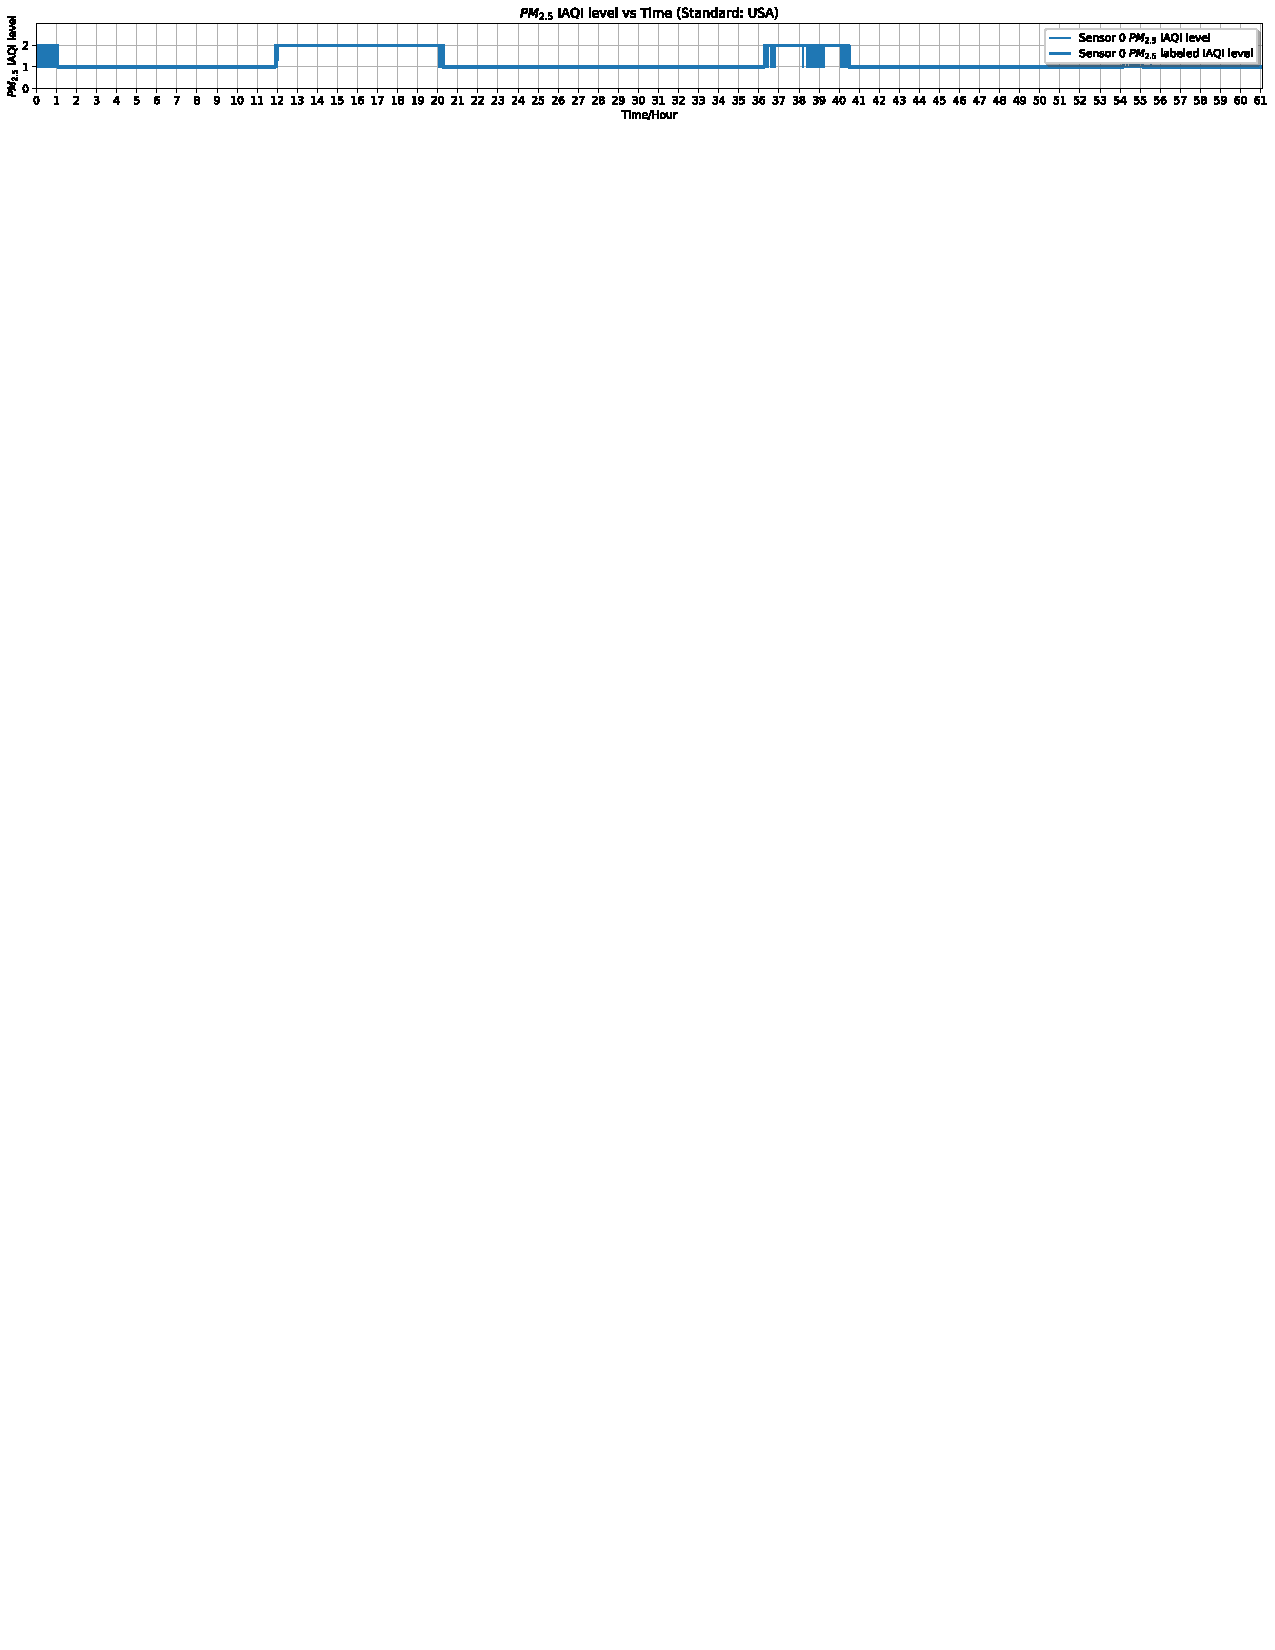
\includegraphics[width=\linewidth]{fig/labeled_iaqi_level/origin_and_labeled/pm25_0.png}
    \end{center}
    \begin{center}
        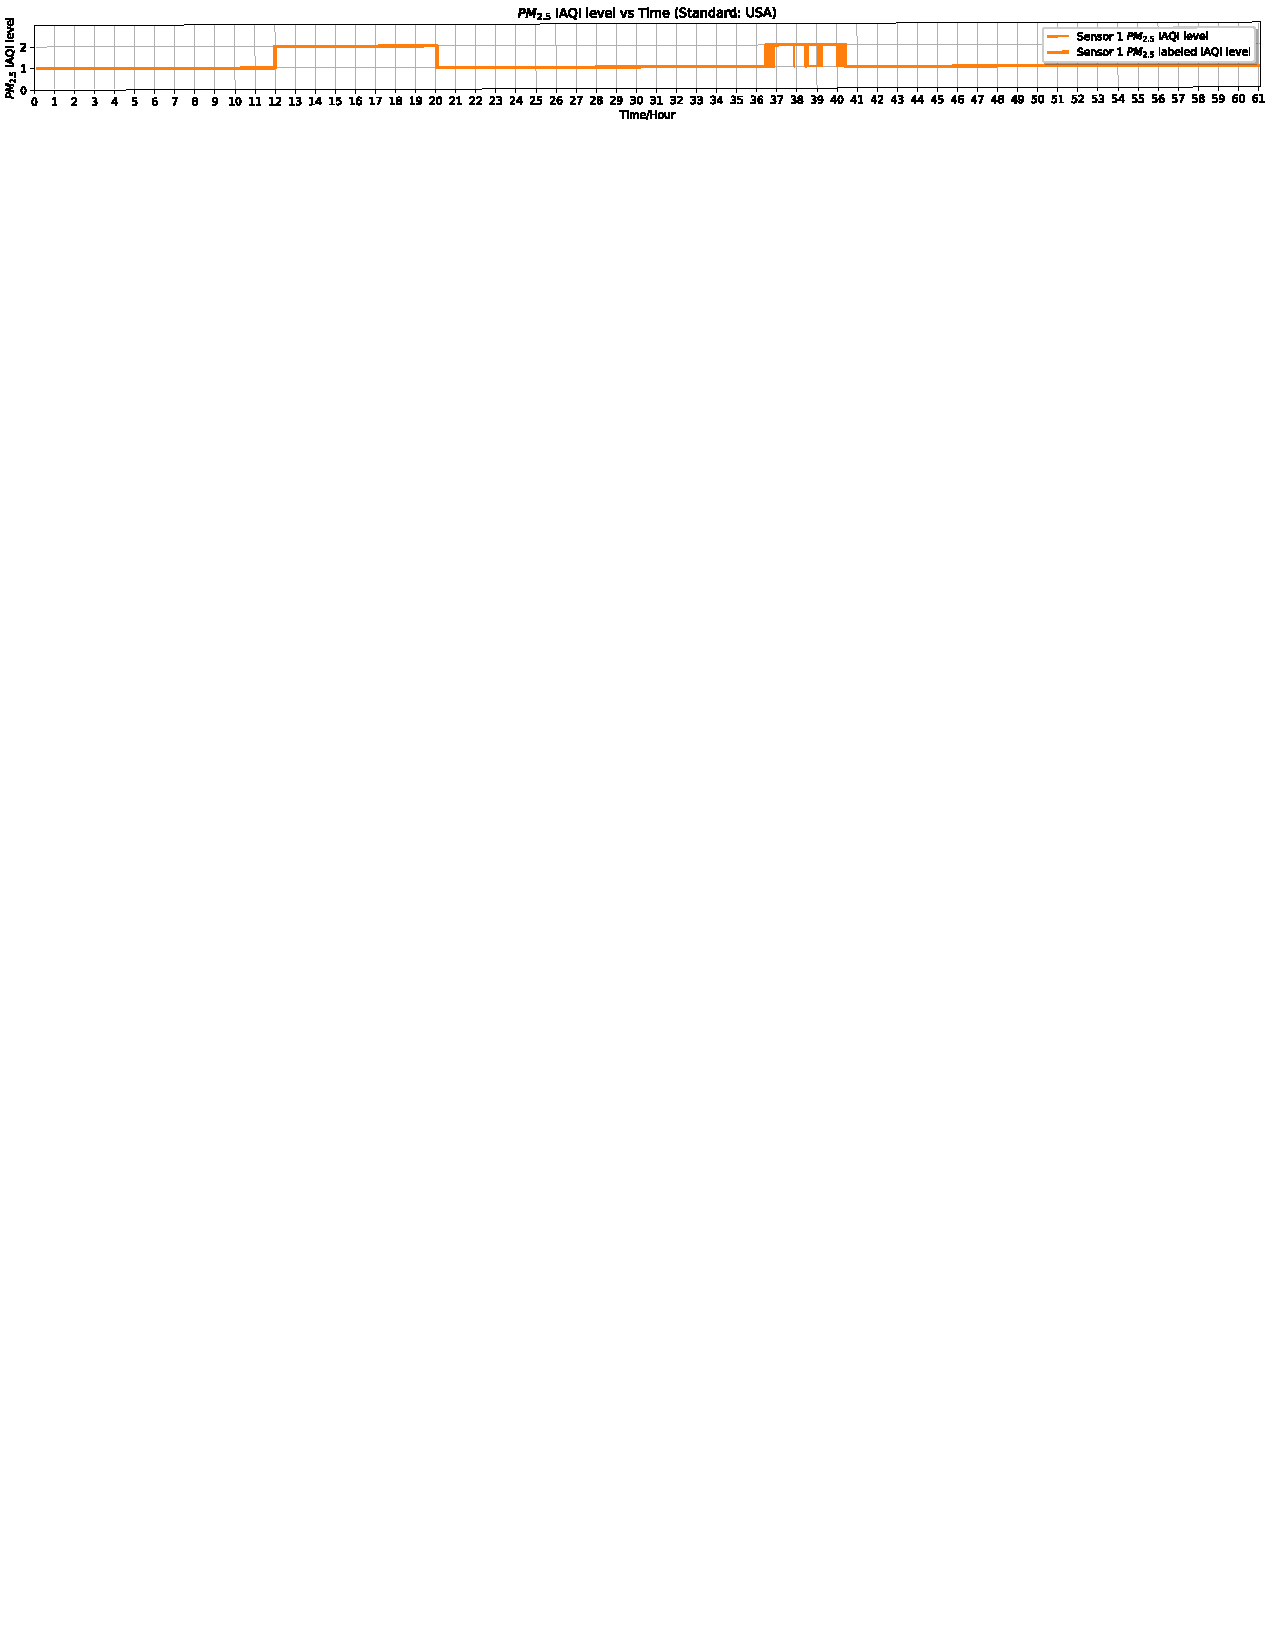
\includegraphics[width=\linewidth]{fig/labeled_iaqi_level/origin_and_labeled/pm25_1.png}
    \end{center}
    \begin{center}
        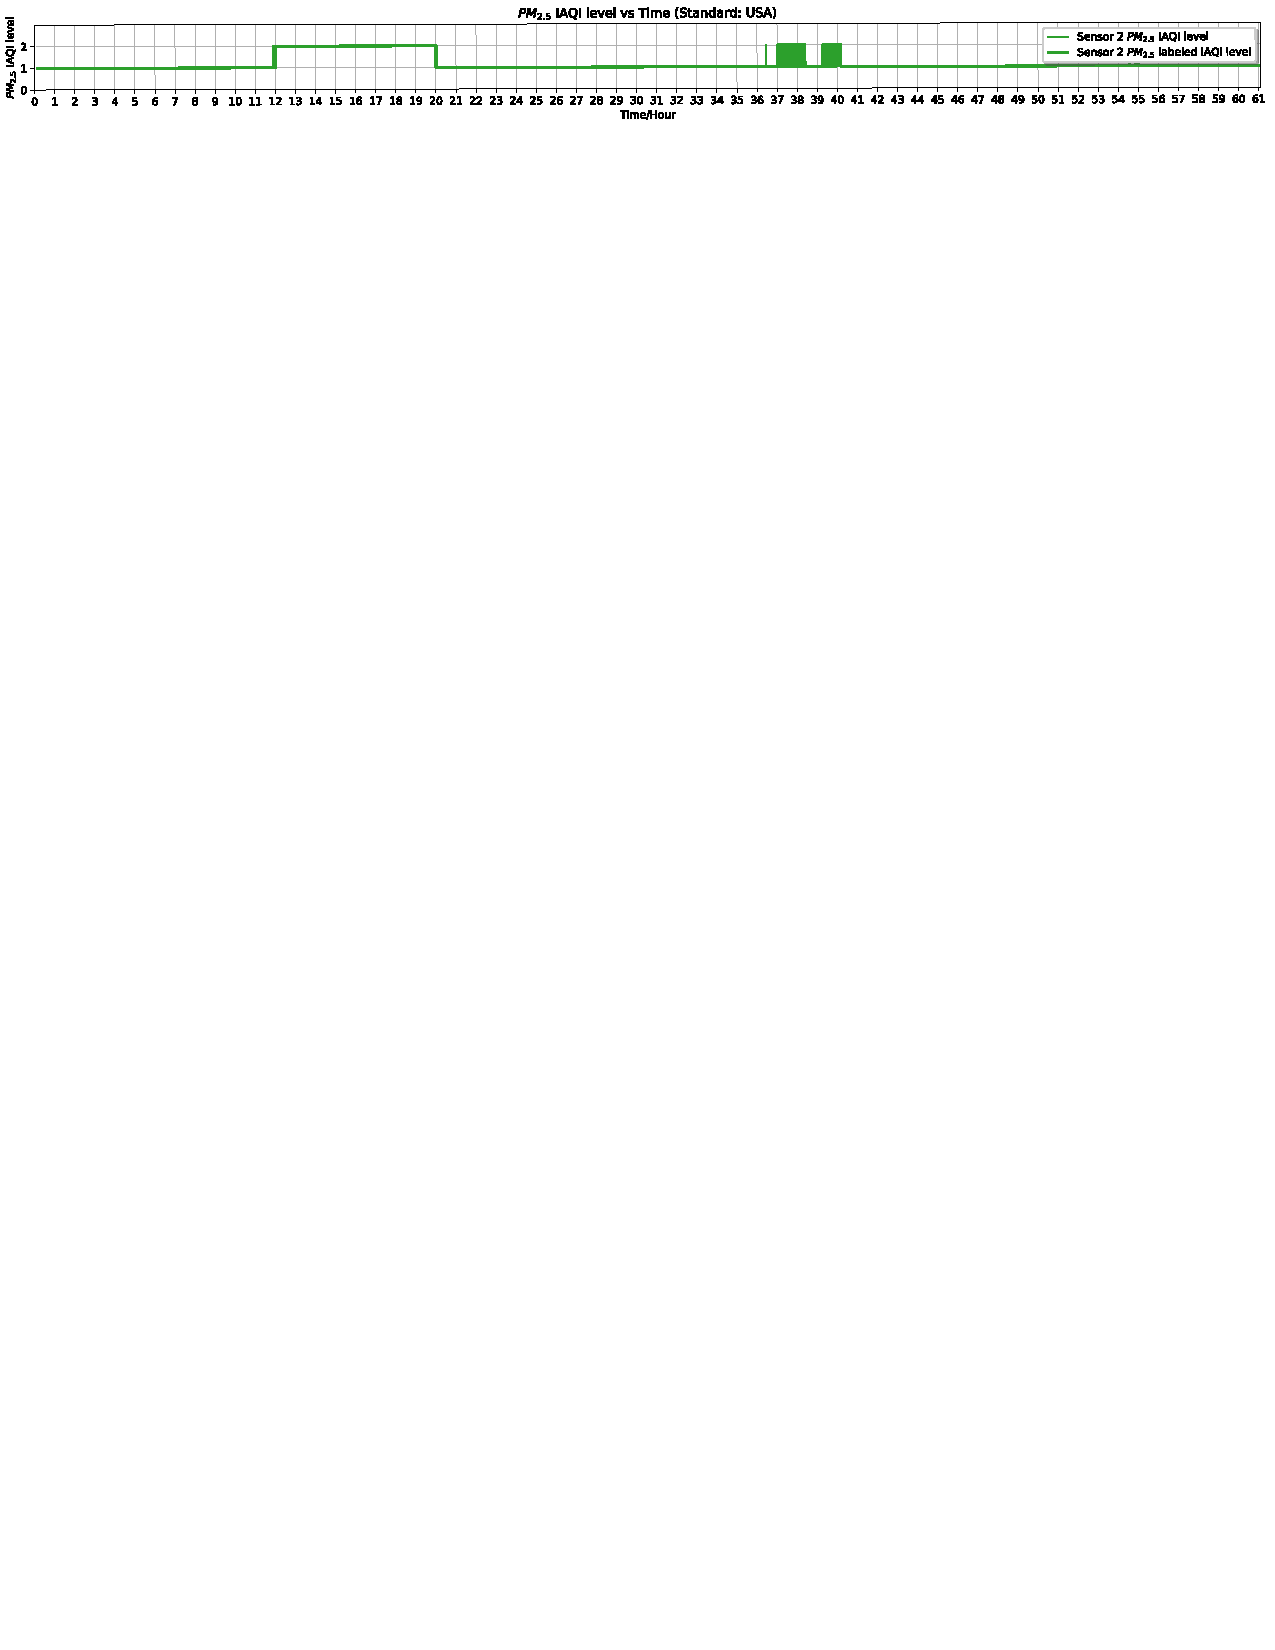
\includegraphics[width=\linewidth]{fig/labeled_iaqi_level/origin_and_labeled/pm25_2.png}
    \end{center}
    \begin{center}
        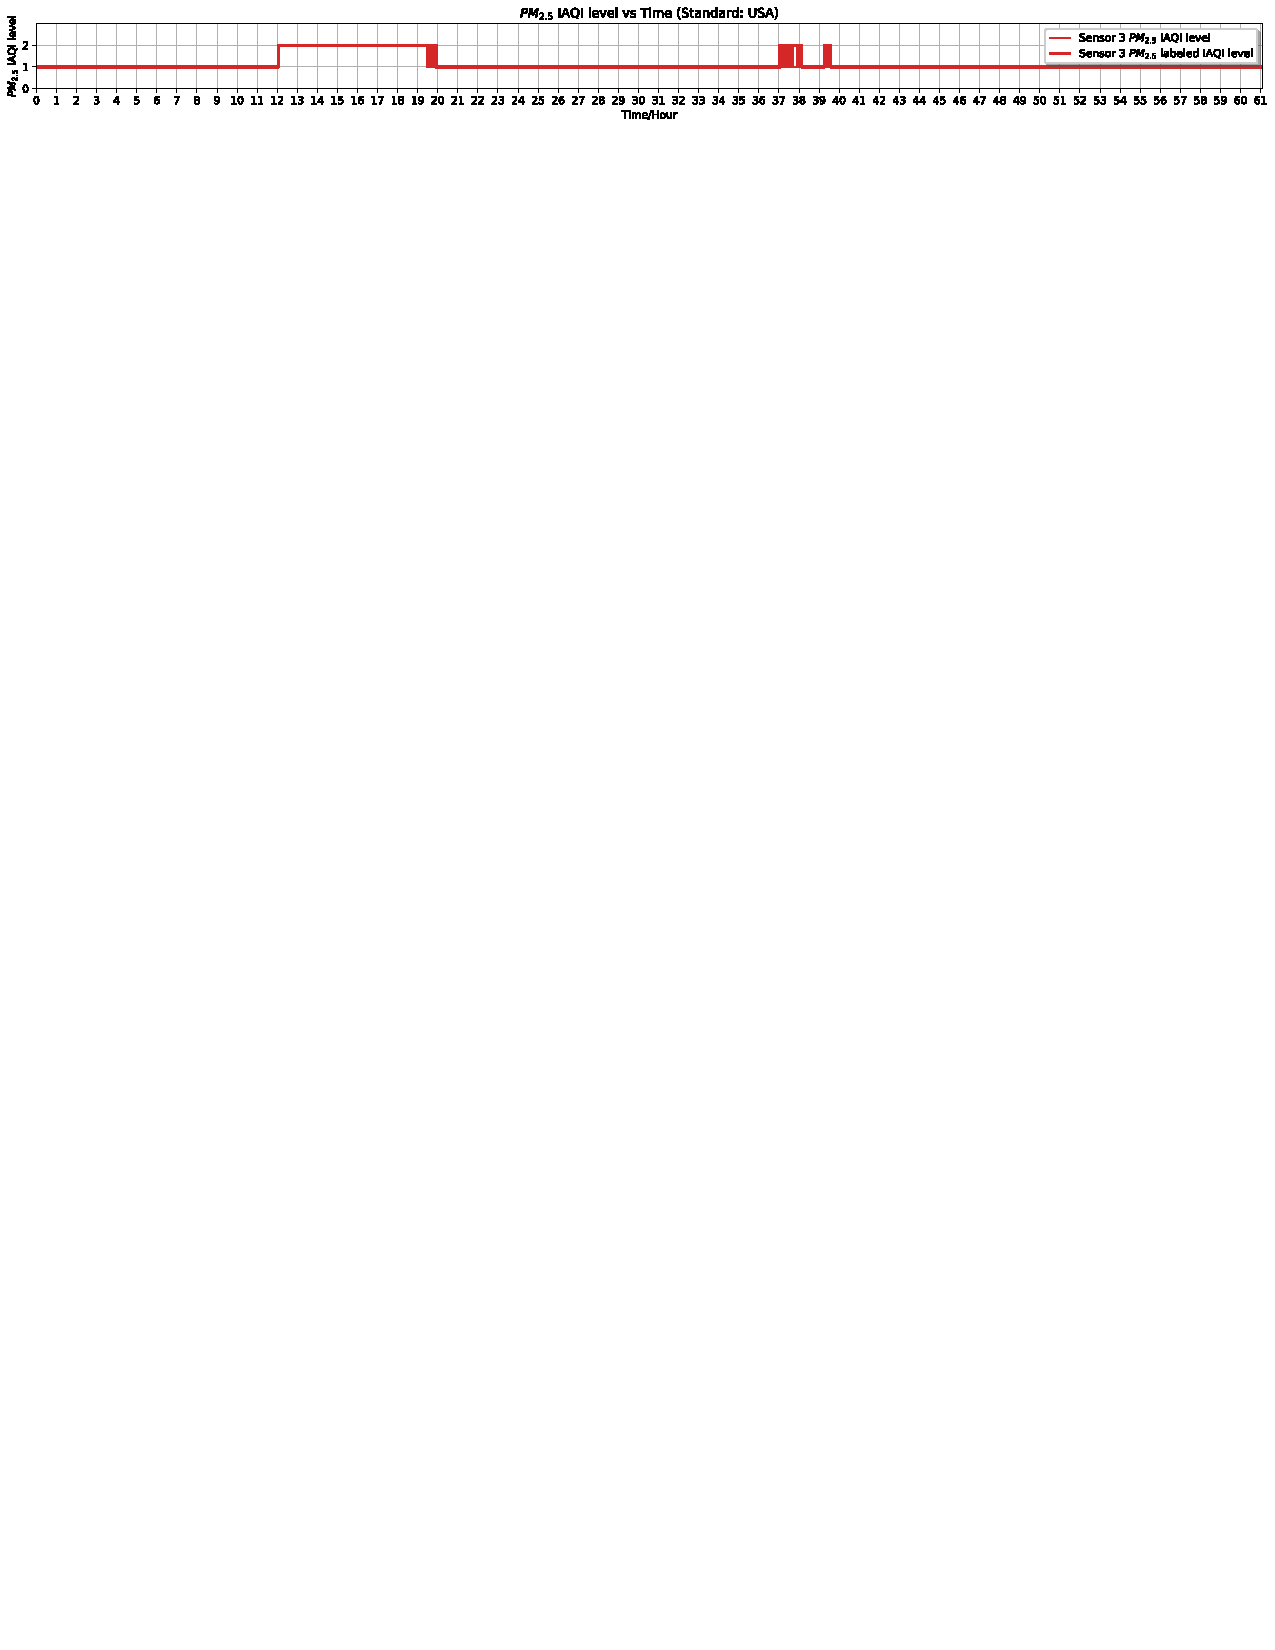
\includegraphics[width=\linewidth]{fig/labeled_iaqi_level/origin_and_labeled/pm25_3.png}
    \end{center}
    \caption{All labeled $PM_{2.5}$ IAQI level.}
    \label{fig:appendix:all_pm25_iaqi_level_and_labeled}
\end{figure}

Figure \ref{fig:appendix:all_pm25_polygonalized_iaqi_level} shows the results of yielding all polygonalized IAQI level lines from the labeled IAQI level.

\begin{figure}[!htbp]
    \begin{center}
        \includegraphics[width=\linewidth]{fig/labeled_iaqi_level/pm25_0_labeled_iaqi_level.png}
    \end{center}
    \begin{center}
        \includegraphics[width=\linewidth]{fig/labeled_iaqi_level/pm25_1_labeled_iaqi_level.png}
    \end{center}
    \begin{center}
        \includegraphics[width=\linewidth]{fig/labeled_iaqi_level/pm25_2_labeled_iaqi_level.png}
    \end{center}
    \begin{center}
        \includegraphics[width=\linewidth]{fig/labeled_iaqi_level/pm25_3_labeled_iaqi_level.png}
    \end{center}
    \caption{All polygonalized $PM_{2.5}$ IAQI level.}
    \label{fig:appendix:all_pm25_polygonalized_iaqi_level}
\end{figure}

% 多余的
% \chapter{Other Model Training Data}\label{chapter:other_model_training_data}
